\section{AI availability}
\label{sec:settings-feature-ai-availability}

This page decides where AI works in the organization. It calls each AI feature a “place”, such as the writing assistant or the notification summary, and each place has its own decision. Use it to stop a feature that does not suit your work, or to limit a feature to chosen members. It opens for the organization’s owner and for holders of the Administrator role at organization level.

Each place is decided in this order: a rule for that member first, then the “Everyone” rule, then the member’s own choice. With no rule and no choice, the place stays on. The “Assistant” is the exception: it stays off until an administrator turns it on, and this setting does not cover the assistant on WhatsApp.

\begin{rcnote}[Example: Horizon]
The system administrator leaves the writing assistant on “Member’s choice” at ① and keeps the “Assistant” off for everyone at ②. The administrator then presses “Edit rules” at ④ for Sarah Al-Khatib and turns the assistant on for her alone, to try it before a wider rollout.
\end{rcnote}

\begin{figure}[H]
\centering
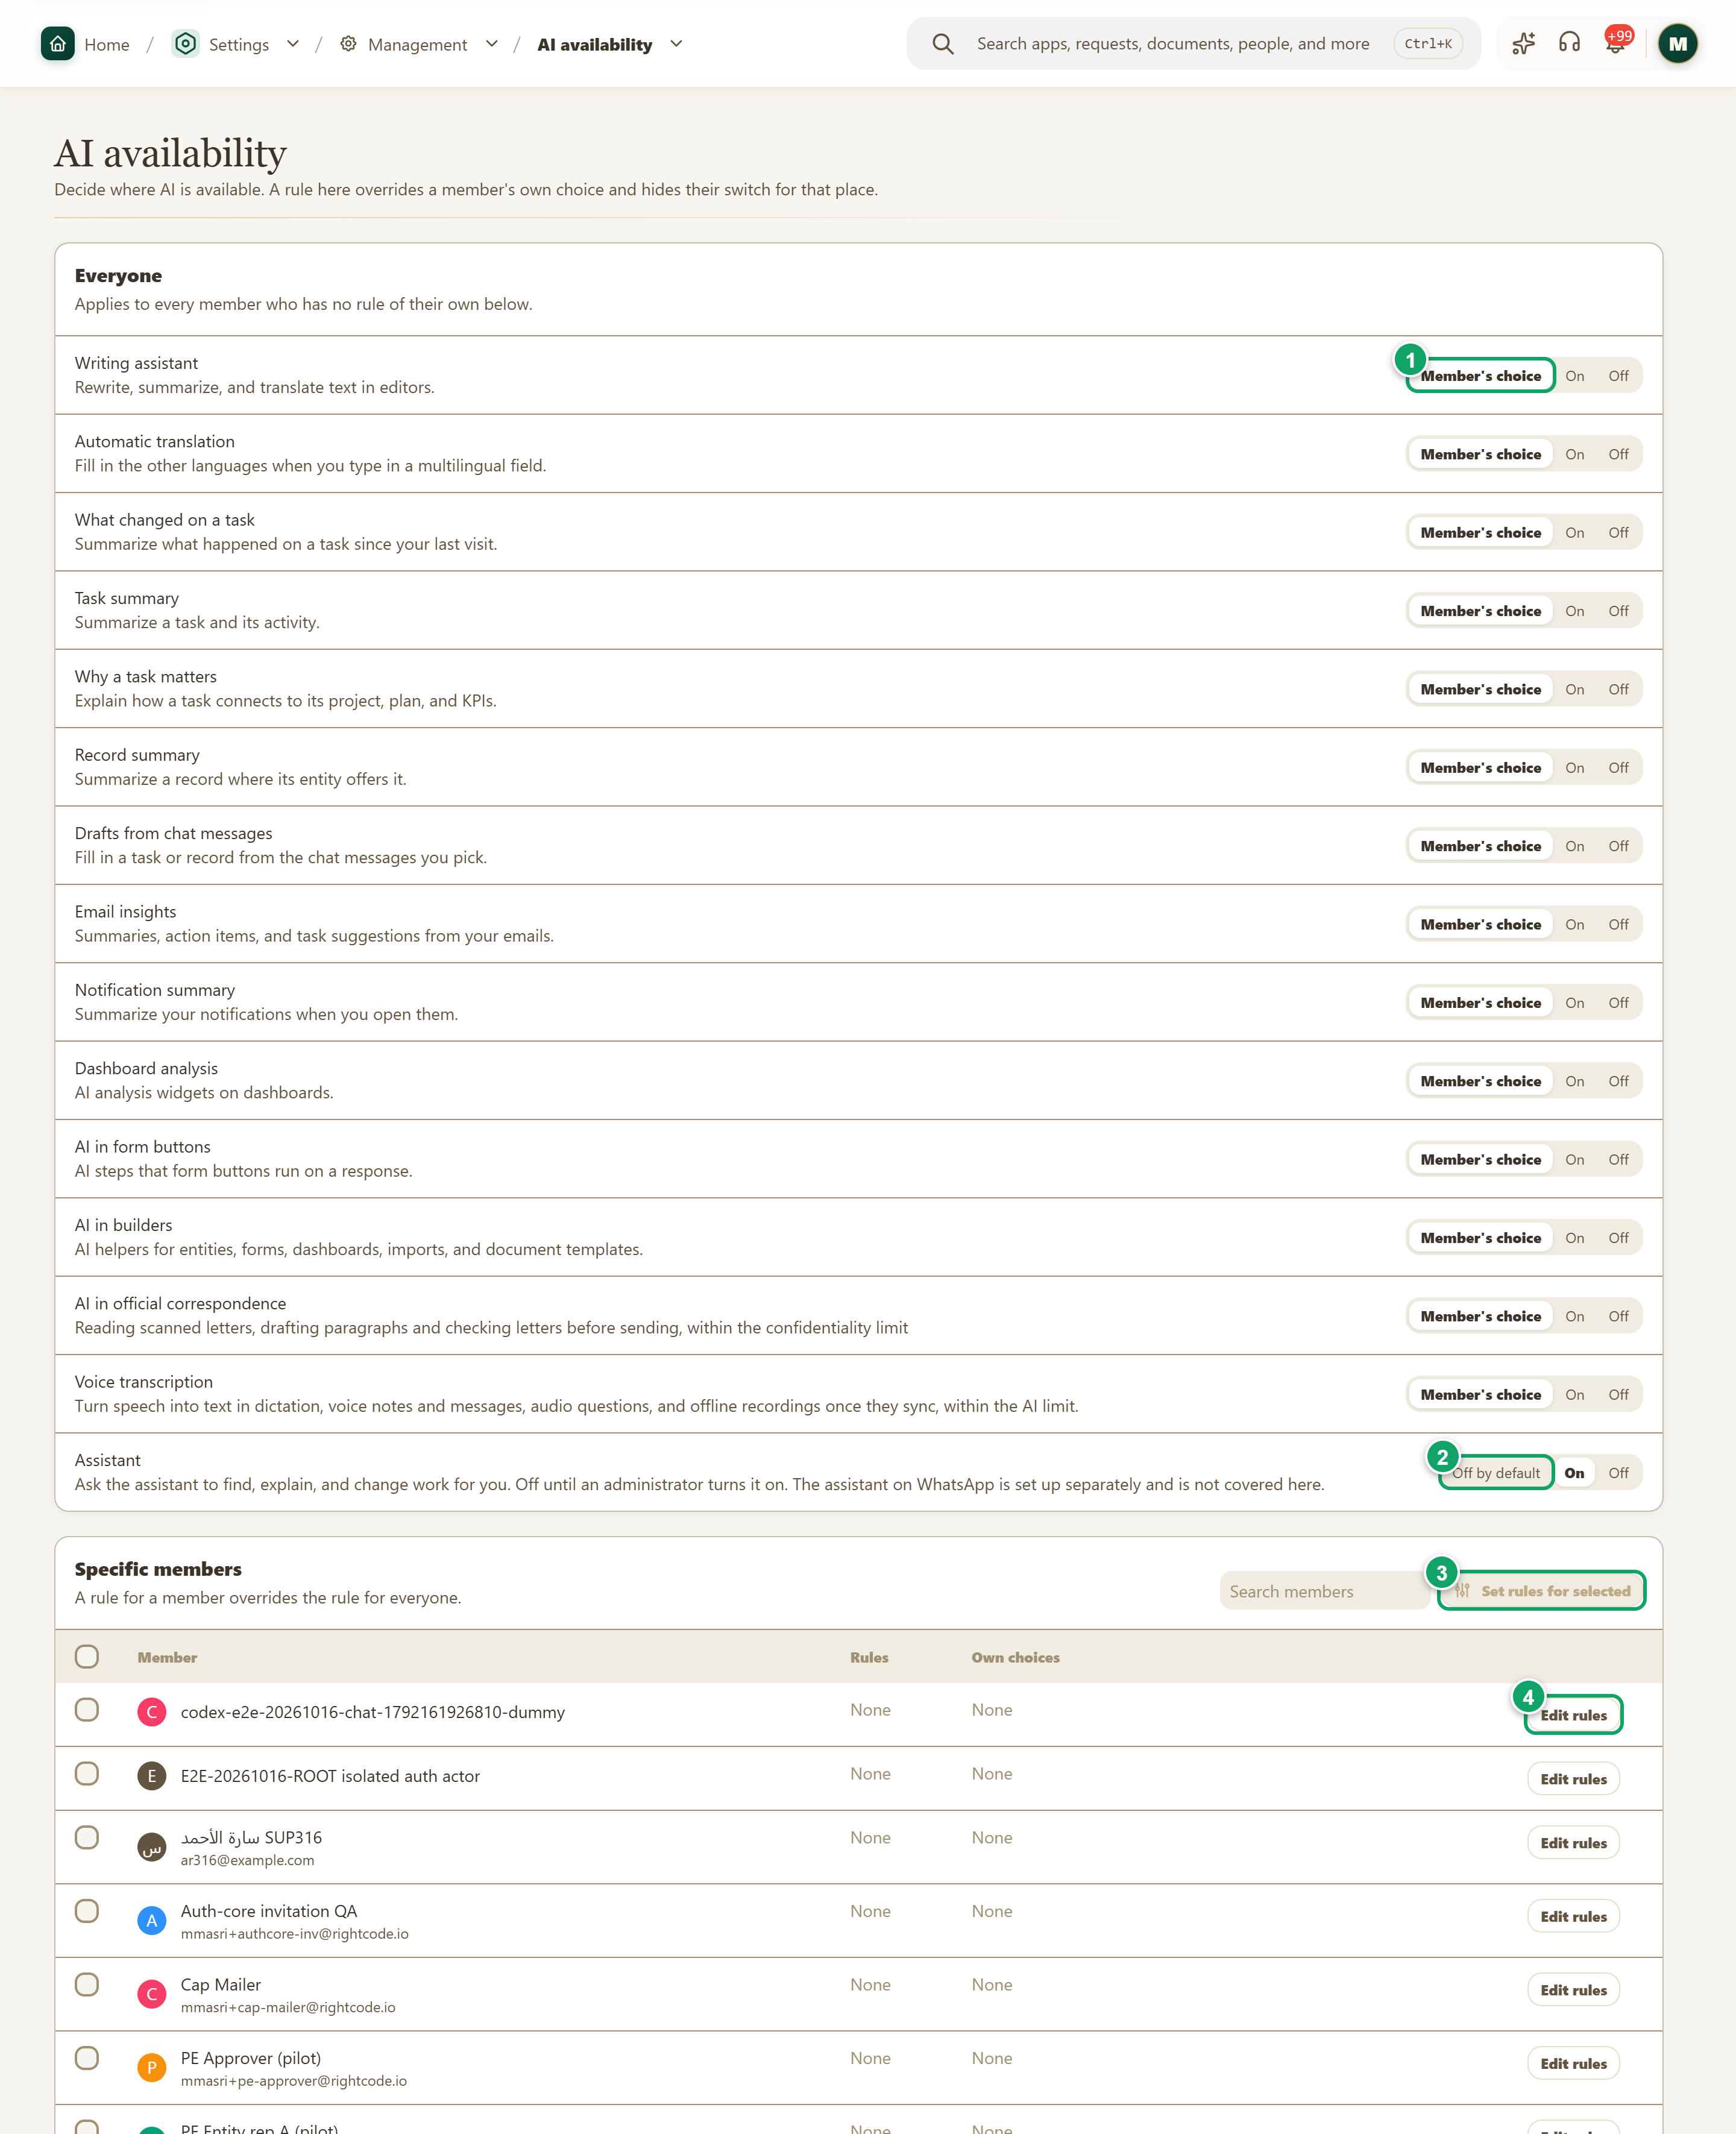
\includegraphics[width=0.95\linewidth,height=0.72\textheight,keepaspectratio]{figures/screens/ch08-ai-availability-en.png}
\caption{Rules for everyone and for specific members}
\label{fig:settings-ai-availability-screen}
\shotnote{The page lists every AI place, with a table below it of the members who can have their own rule. Comparing the “Rules” and “Own choices” columns shows what an administrator imposed and what the member chose. ① “Member’s choice”: leaves the decision to the member; “On” and “Off” beside it impose the decision and hide the member’s switch. ② “Off by default”: replaces “Member’s choice” in the “Assistant” row, because the member does not decide it; the test organization has chosen “On” here. ③ “Set rules for selected”: works once you select one or more members in the table. ④ “Edit rules”: for one member.}
\end{figure}

\begin{table}[H]
\centering
\caption{What do you decide on this page?}
\label{tab:settings-ai-availability-fields}
\begin{tabularx}{\linewidth}{R{4.2cm} Y}
\rcHeaderRow
\thh{Section or option} & \thh{Meaning}\\
“Everyone” & A rule for each place, applied to every member without a rule of their own. It saves as soon as you press it; this section has no save button.\\
“Member’s choice” / “On” / “Off” & The first leaves the decision to the member in their account settings. The other two lock the place, and the system ignores the member’s choice.\\
“Specific members” & A rule for one or more members that overrides the “Everyone” rule. Find members by searching their name or email.\\
“Rules” & The places where an administrator set a rule for this member.\\
“Own choices” & What the member chose personally. It stays saved even while a rule overrides it, and applies again once the rule is removed.\\
\end{tabularx}
\end{table}

\begin{figure}[H]
\centering
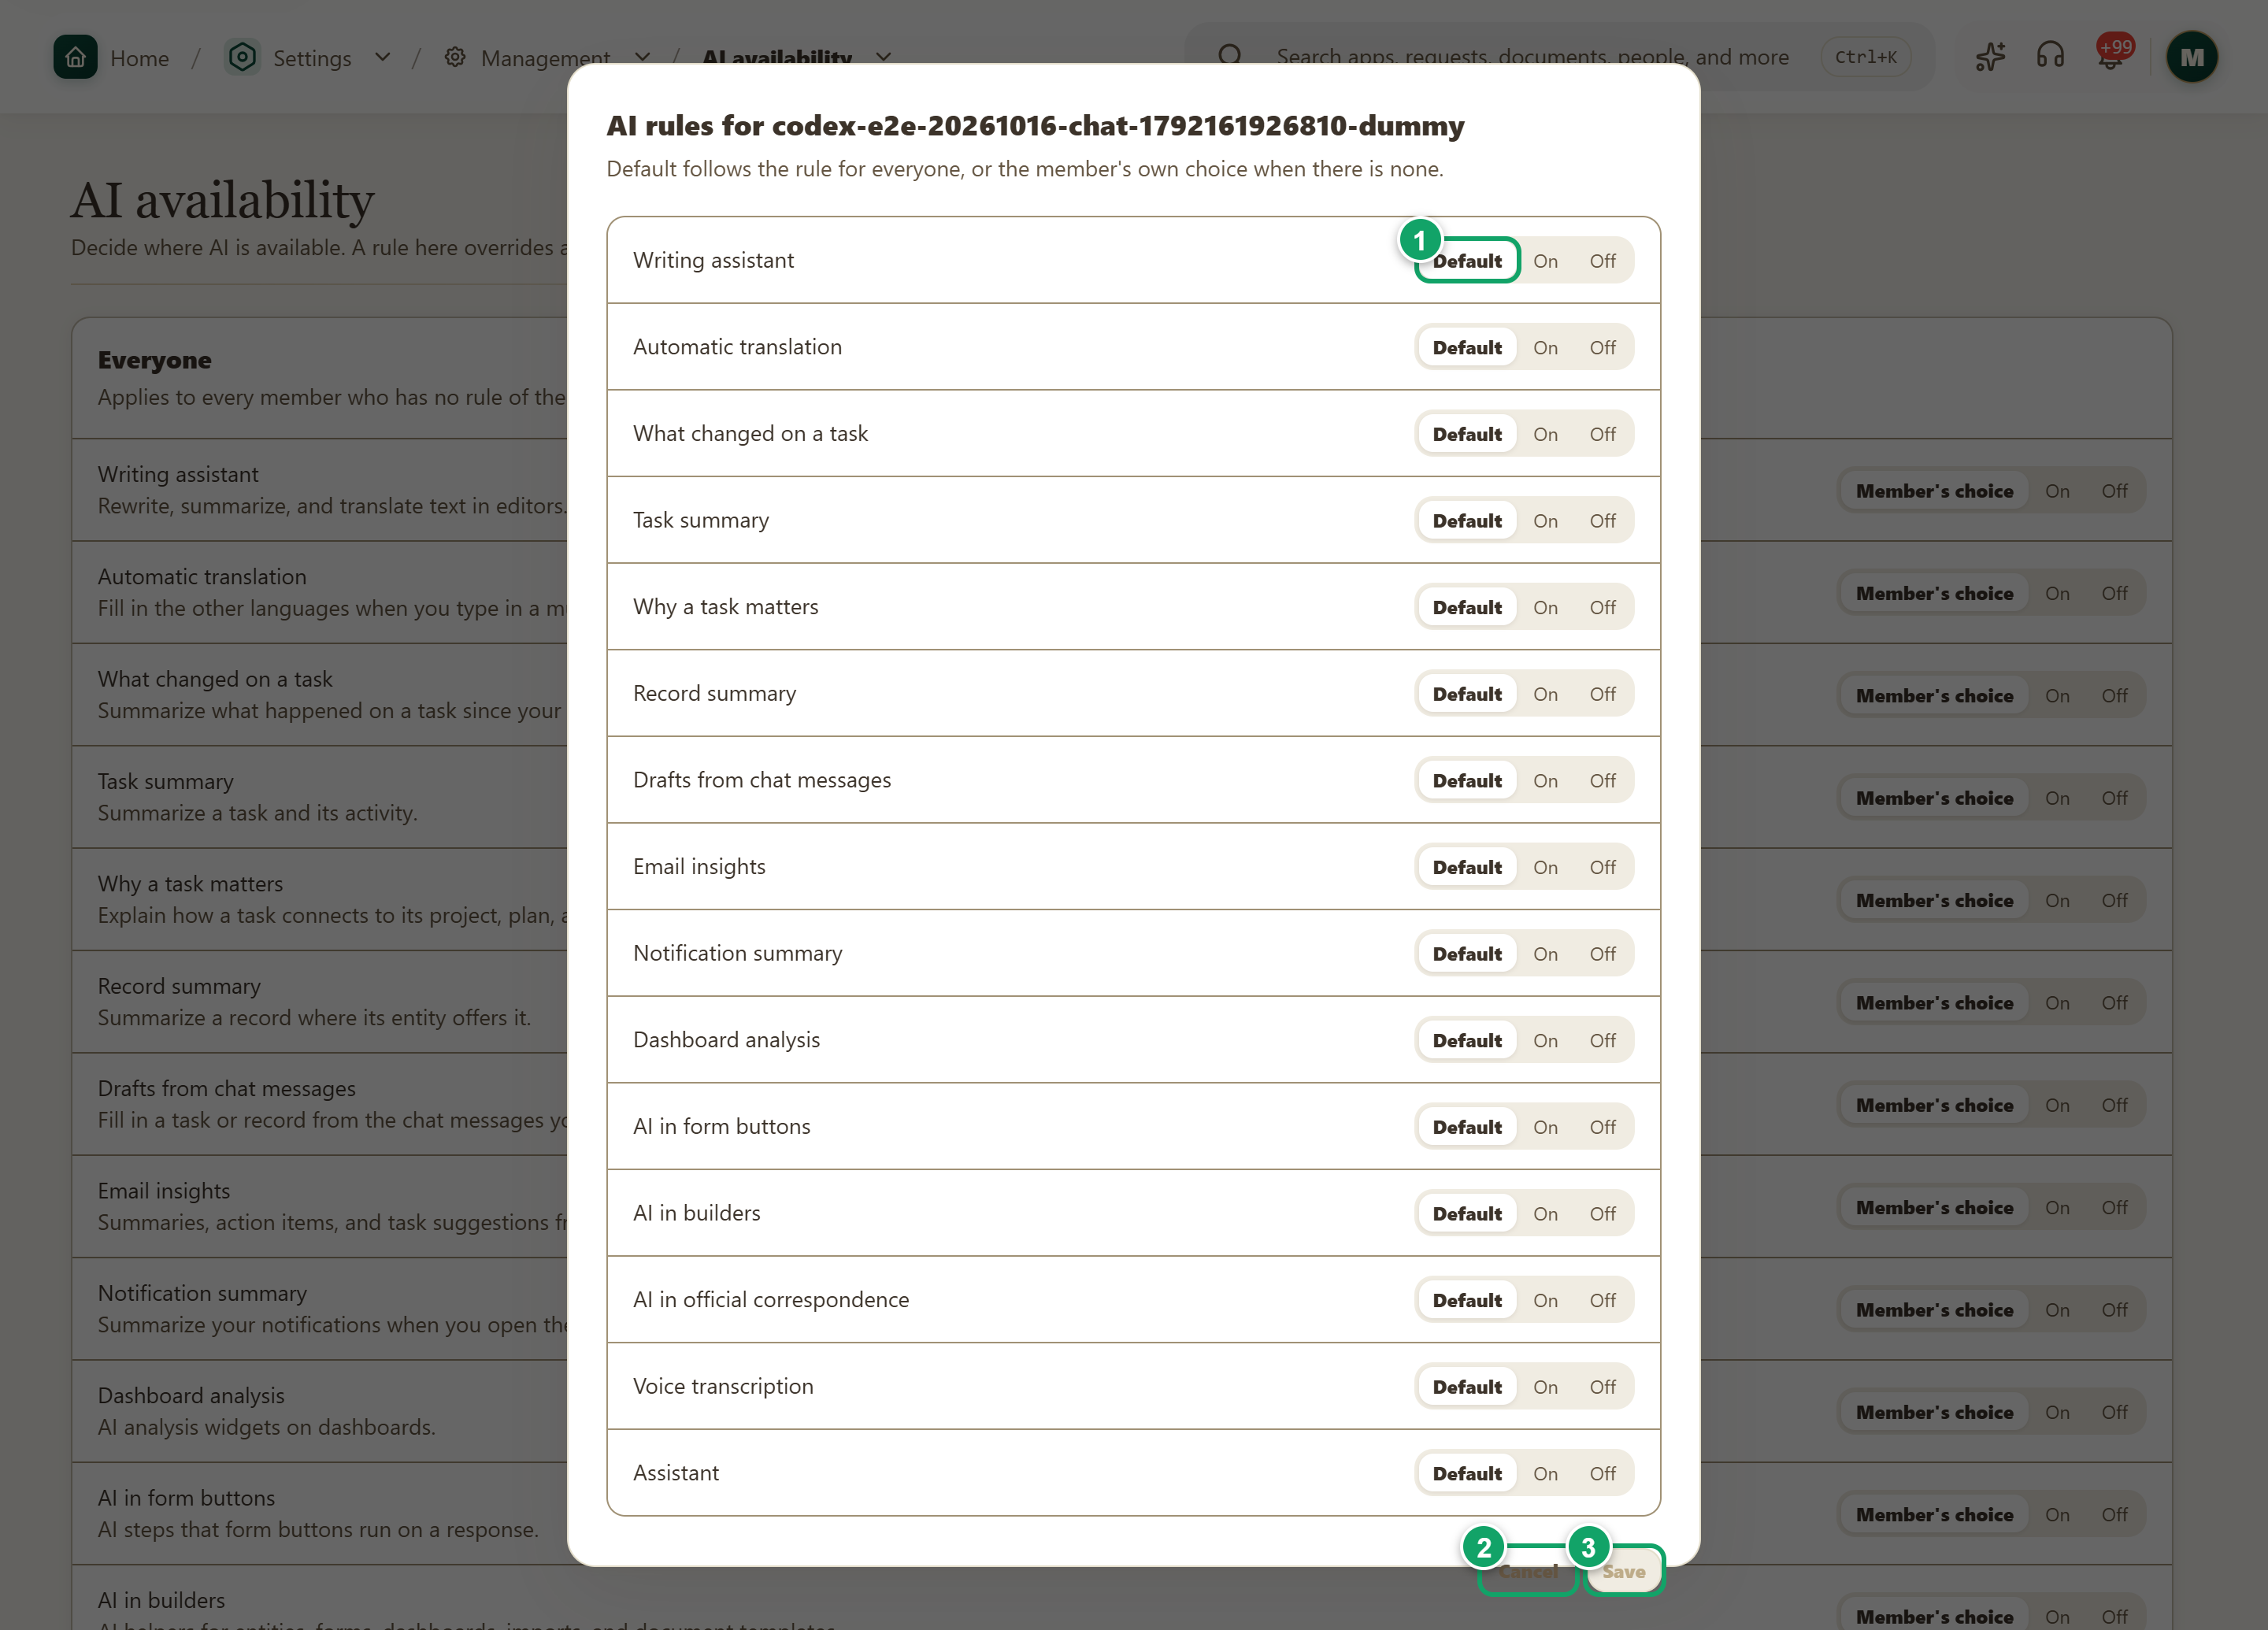
\includegraphics[width=0.95\linewidth,height=0.72\textheight,keepaspectratio]{figures/screens/ch08-ai-availability-member-en.png}
\caption{AI rules for a member}
\label{fig:settings-ai-availability-member-screen}
\shotnote{The window shows the same places for one member or for a selected group. With several members, only the place you changed is touched, so their other rules stay as they are. ① “Default”: follows the “Everyone” rule, or the member’s choice when there is none. ② “Cancel”: closes without changes. ③ “Save”: stays disabled until you change at least one rule.}
\end{figure}

\begin{enumerate}
\item Open “Settings”, then “AI availability”.
\item In the “Everyone” section, pick the value for each place. Remember that your choice saves at once.
\item To set a rule for one member, press “Edit rules” in their row. For several members, select them and press “Set rules for selected”.
\item Choose “On” or “Off” for the place, then press “Save”.
\end{enumerate}

\textbf{Check:} The message “AI availability saved.” appears, and the “Rules” column shows the place and its state for that member. When the member opens their account settings, the switch for that place is gone. If a feature is still missing for a member after you turned it on, check their own rule first, because it comes before the “Everyone” rule, then look at “AI limits”.

\section{AI limits}
\label{sec:settings-feature-ai-limits}

This page sets the budget that AI consumes and shows how much of it is used. Every AI request has a cost, recorded in US dollars. It is deducted from the member’s allowance when a member asks for it, and from the “Full organization allowance” when it is not tied to a member. Use the page to keep within budget and to see which features cost the most. It opens for the organization’s owner and for holders of the Administrator role at organization level.

A limit is a fixed amount that does not renew by itself each month. Raising it adds the difference to “Remaining”; lowering it takes the difference away. When the balance runs out, the system refuses new AI requests charged to that balance until the limit is raised.

\begin{rcnote}[Example: Horizon]
The system administrator notices that Omar Haddad’s balance is “Low” and looks for the feature that used it at ②. The administrator then selects Omar’s row in the table, types a new limit at ③ and presses “Apply limit” at ④.
\end{rcnote}

\begin{figure}[H]
\centering
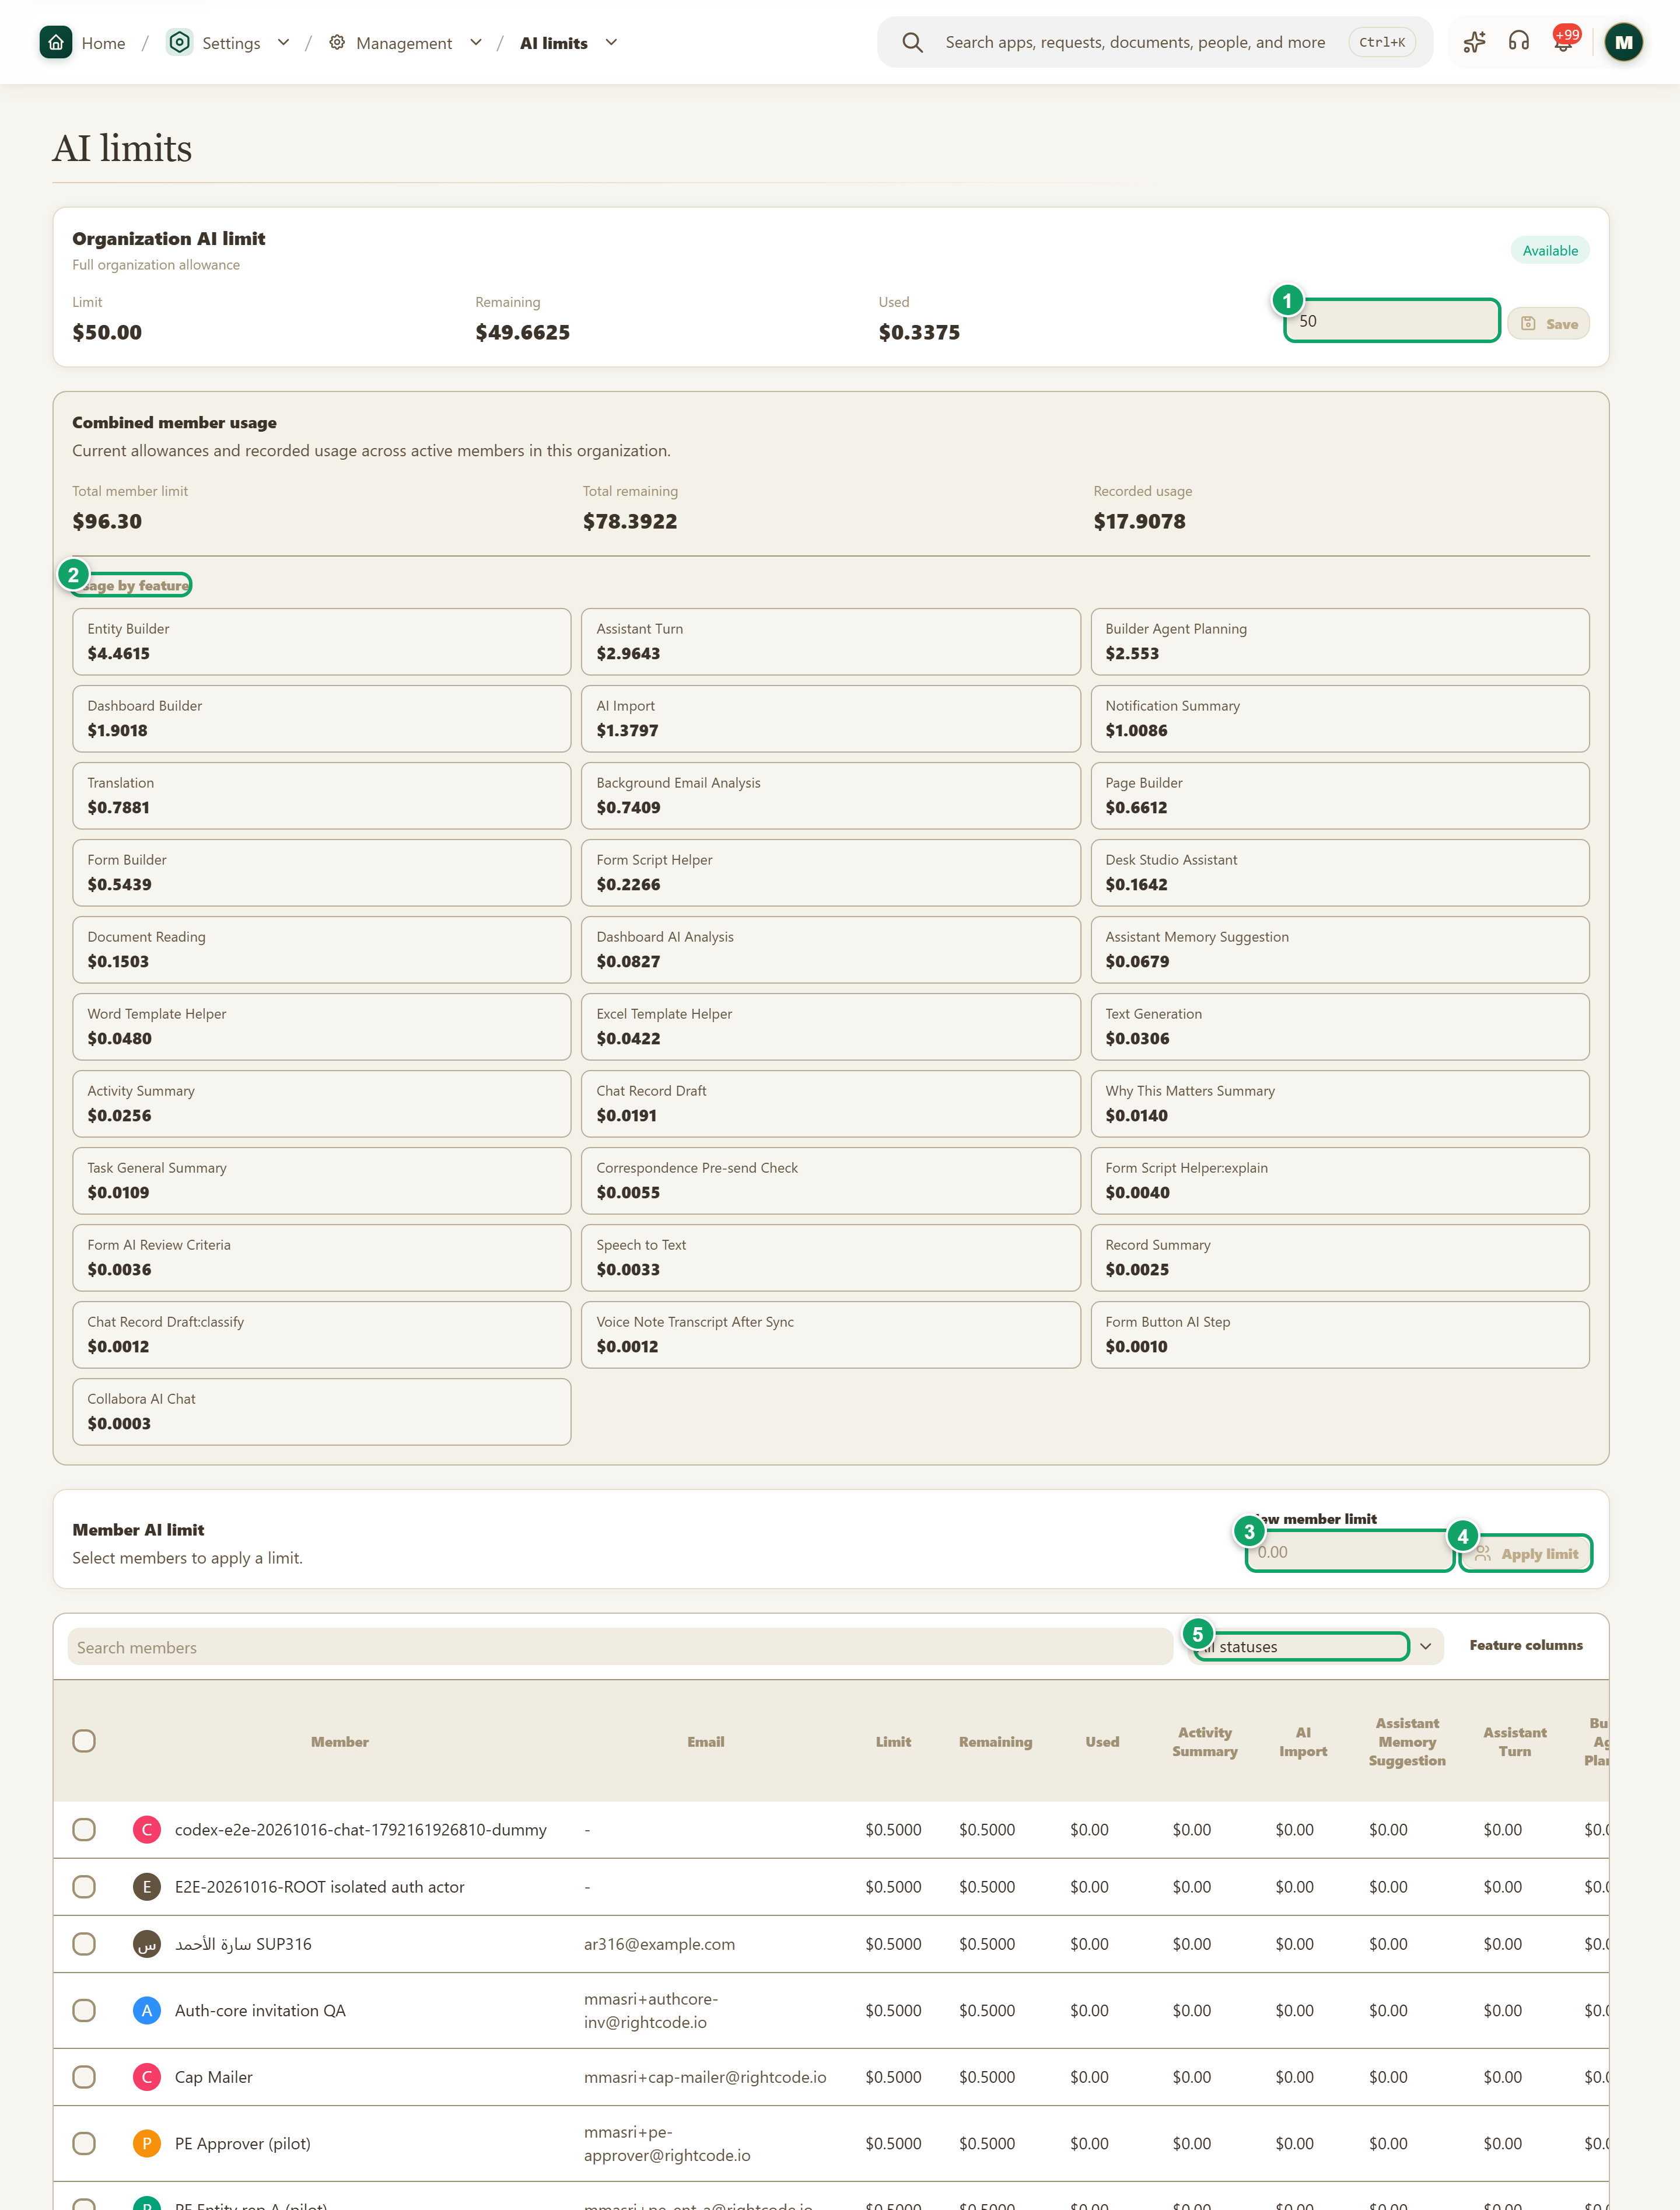
\includegraphics[width=0.95\linewidth,height=0.72\textheight,keepaspectratio]{figures/screens/ch08-ai-limits-en.png}
\caption{The organization limit, member limits and usage}
\label{fig:settings-ai-limits-screen}
\shotnote{The image shows the organization allowance, then the total of member limits and usage, then a table with one row per member. The figures belong to the test organization. The difference between the parts matters: changing the organization limit does not change member limits, and changing a member’s limit does not touch the organization allowance. ① The organization limit field, saved with “Save” beside it. ② “Usage by feature”: shows where the cost went. ③ “New member limit”. ④ “Apply limit”: works once a member is selected and the value is valid. ⑤ “All statuses”: filters the table by balance state.}
\end{figure}

\begin{table}[H]
\centering
\caption{What do you read and record on this page?}
\label{tab:settings-ai-limits-fields}
\begin{tabularx}{\linewidth}{R{4.2cm} Y}
\rcHeaderRow
\thh{Section} & \thh{What it shows or records}\\
“Organization AI limit” & “Limit”, “Remaining” and “Used” for the organization allowance, with a field to change the limit.\\
“Combined member usage” & “Total member limit”, “Total remaining” and “Recorded usage” for active members, then the cost per feature.\\
“Member AI limit” & One limit applied at once to the selected members.\\
Member table & Email, limit, remaining and used for each member. “Feature columns” adds the cost per feature.\\
“Status” & “Available” while there is balance, “Low” when less than 20\% of the limit remains, and “Exhausted” when the balance is gone.\\
\end{tabularx}
\end{table}

\begin{enumerate}
\item Open “Settings”, then “AI limits”.
\item To change the organization allowance, type the value in the limit field and press “Save”.
\item To change member limits, select their rows in the table. You can search or filter by status first.
\item Type the value in “New member limit”, then press “Apply limit”.
\end{enumerate}

\textbf{Check:} The message “AI limits saved.” appears, “Limit” and “Remaining” in that row change by the difference, and “Status” updates. The field rejects letters and negative values: it shows an error color and nothing saves.
